% =============================================================================
% Monocular 3D Object Detection: Training Pipeline Description
% Prepared for ECCV Submission
% =============================================================================

\documentclass[runningheads]{llncs}

\usepackage{amsmath,amssymb}
\usepackage{graphicx}
\usepackage{booktabs}
\usepackage{algorithm}
\usepackage{algorithmic}
\usepackage{xcolor}
\usepackage{hyperref}
\usepackage{multirow}
\usepackage{tikz}
\usetikzlibrary{shapes.geometric, arrows.meta, positioning, fit, backgrounds}

\begin{document}

\title{Monocular 3D Object Detection via DINOv2-Backed\\Factorized Regression with OVMono3D Supervision}

\author{}
\institute{}

\maketitle

% =============================================================================
\section{Monocular 3D Object Detection Pipeline}
\label{sec:mono3d_pipeline}
% =============================================================================

We present a monocular 3D object detection framework that lifts standard 2D bounding box detection into calibrated 3D space using a single RGB image.
The system is built upon a frozen DINOv2~\cite{oquab2024dinov2} Vision Transformer backbone, augmented with a Simple Feature Pyramid Network (SimpleFPN) adapted from ViTDet~\cite{li2022vitdet}, a Faster R-CNN~\cite{ren2015fasterrcnn} detection head for 2D object localization, and a novel \textbf{Factorized Monocular 3D Head} that performs disentangled regression of 3D bounding box parameters.
The full training pipeline is summarized in Figure~\ref{fig:pipeline_overview}.

\begin{figure}[t]
\centering
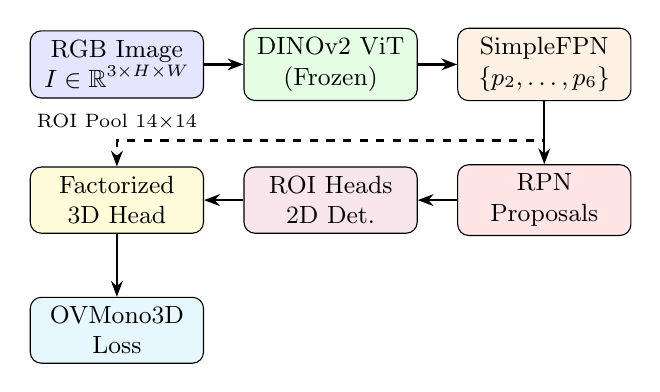
\begin{tikzpicture}[
    node distance=0.8cm and 0.5cm,
    block/.style={rectangle, draw, rounded corners, minimum height=0.8cm, minimum width=2.2cm, align=center, font=\small},
    arrow/.style={-{Stealth[length=2mm]}, thick},
]
% Nodes
\node[block, fill=blue!10] (img) {RGB Image\\$I \in \mathbb{R}^{3 \times H \times W}$};
\node[block, fill=green!10, right=of img] (backbone) {DINOv2 ViT\\(Frozen)};
\node[block, fill=orange!10, right=of backbone] (fpn) {SimpleFPN\\$\{p_2,\ldots,p_6\}$};
\node[block, fill=red!10, below=of fpn] (rpn) {RPN\\Proposals};
\node[block, fill=purple!10, left=of rpn] (roi) {ROI Heads\\2D Det.};
\node[block, fill=yellow!15, left=of roi] (head3d) {Factorized\\3D Head};
\node[block, fill=cyan!10, below=of head3d] (loss) {OVMono3D\\Loss};
% Arrows
\draw[arrow] (img) -- (backbone);
\draw[arrow] (backbone) -- (fpn);
\draw[arrow] (fpn) -- (rpn);
\draw[arrow] (rpn) -- (roi);
\draw[arrow] (roi) -- (head3d);
\draw[arrow] (head3d) -- (loss);
\draw[arrow, dashed] (fpn.south) -- ++(0,-0.5) -| (head3d.north) node[midway, above, font=\scriptsize] {ROI Pool 14$\times$14};
\end{tikzpicture}
\caption{\textbf{Pipeline overview.} The forward pass proceeds through six stages: image batching, frozen backbone feature extraction, multi-scale feature pyramid construction, region proposal generation, 2D detection, and factorized 3D bounding box regression. During training, the OVMono3D loss provides geometry-level disentangled supervision.}
\label{fig:pipeline_overview}
\end{figure}


% =============================================================================
\subsection{Dataset Preparation and Preprocessing}
\label{sec:dataset}
% =============================================================================

\subsubsection{Action Genome 3D Dataset.}
We train our detector on the Action Genome~\cite{ji2020actiongenome} dataset, which provides frame-level annotations for 37 object categories (plus background) across approximately 10K video clips.
Each frame is annotated with person bounding boxes and per-object 2D bounding boxes in $[x_1, y_1, x_2, y_2]$ format, along with class labels and visibility flags.
We extend these annotations with 3D ground truth in the form of 8-corner world-coordinate bounding boxes $(8 \times 3)$ for each annotated object, stored as per-video pickle files.

\subsubsection{Frame Indexing and Filtering.}
During dataset construction, we iterate over all annotated frames and build a per-frame sample index.
Frames that lack person bounding boxes are filtered when \texttt{filter\_nonperson\_box\_frame} is enabled, ensuring that all training samples contain at least one person detection.
For each remaining frame, we collect all visible objects with valid bounding boxes and record their class indices and 2D box coordinates.
The resulting sample index maps each frame to its person boxes, object boxes, 3D corner annotations, and associated metadata.

\subsubsection{3D Ground Truth Loading.}
The 3D annotations are loaded from per-video pickle files that store oriented bounding box corners in world coordinates.
We support three annotation formats: (i) axis-aligned floor bounding boxes (\texttt{aabb\_floor\_aligned/corners\_world}), (ii) top-level world corners (\texttt{corners\_world}), and (iii) oriented bounding box corners (\texttt{obb\_corners\_final}).
A compatibility unpickler handles numpy version mismatches (numpy 2.x pickles loaded on numpy 1.x) by transparently redirecting \texttt{numpy.\_core} to \texttt{numpy.core}.
During sample retrieval, each 2D object is matched to its corresponding 3D annotation by class index; unmatched objects receive zero-padded 3D corners $(8 \times 3)$ that are filtered out during loss computation.

\subsubsection{Resolution-Aware Preprocessing.}
\label{sec:resolution_bucketing}
A critical design choice in our pipeline is \textbf{resolution bucketing}, which enables efficient batching of images with diverse aspect ratios without padding waste.
At dataset initialization, we compute the target resolution for each video (not each frame, since all frames within a video share the same native resolution):

\begin{enumerate}
    \item \textbf{Native resolution reading}: We read only the image header (JPEG SOF marker or PNG IHDR chunk) to extract the native width $W_o$ and height $H_o$ without decoding the full image, yielding a $25\times$ speedup over PIL-based dimension reading.
    
    \item \textbf{Aspect-ratio-preserving resize}: Given a pixel budget $P = 255{,}000$ (chosen to balance GPU memory and feature resolution), we compute a scale factor $s = \sqrt{P / (W_o \cdot H_o)}$ and derive target dimensions:
    \begin{equation}
        W_t = k \cdot p, \quad H_t = m \cdot p, \quad \text{s.t.} \quad k = \text{round}\!\left(\frac{W_o \cdot s}{p}\right), \quad m = \text{round}\!\left(\frac{H_o \cdot s}{p}\right)
    \end{equation}
    where $p = 14$ is the ViT patch size. The constraint $W_t \cdot H_t \leq P$ is enforced by iteratively decrementing $k$ or $m$ along the dimension with greater relative excess. This ensures all images are exact multiples of the patch size, eliminating fractional patches.
    
    \item \textbf{Bucket assignment}: Frames sharing the same $(W_t, H_t)$ are grouped into resolution buckets. The batch sampler draws all samples within a batch from the same bucket, guaranteeing that \texttt{torch.stack} succeeds without padding while allowing frames from \emph{different} videos in the same batch, maximizing gradient diversity.
\end{enumerate}

\subsubsection{Per-Frame Data Pipeline.}
At training time, each \texttt{\_\_getitem\_\_} call executes the following pipeline:

\begin{enumerate}
    \item \textbf{Image decoding}: The RGB frame is loaded via \texttt{torchvision.io.read\_image} (hardware-accelerated JPEG decoding) as a uint8 CHW tensor, or falls back to PIL if unavailable.
    
    \item \textbf{Deterministic resize}: The image is bilinearly interpolated to the pre-computed $(W_t, H_t)$ with anti-aliasing, then converted to float32 in $[0, 1]$.
    
    \item \textbf{DINOv2 normalization}: Channel-wise normalization with ImageNet statistics ($\mu = [0.485, 0.456, 0.406]$, $\sigma = [0.229, 0.224, 0.225]$) is applied in-dataset rather than in the model transform, enabling the model's \texttt{GeneralizedRCNNTransform} to be a pure batching pass-through (no resize, no normalize).
    
    \item \textbf{Bounding box scaling}: All 2D boxes are scaled by $(s_x, s_y) = (W_t / W_o, H_t / H_o)$ and clamped to image boundaries. Degenerate boxes (width or height $< 1$ pixel) are discarded.
    
    \item \textbf{Camera intrinsics}: Per-video camera intrinsics $(f_x, f_y, c_x, c_y)$ are loaded if available; otherwise, a default pinhole model is constructed with $f_x = f_y = \max(W_t, H_t)$ and principal point at the image center. Intrinsics are scaled by the same $(s_x, s_y)$ factors to remain consistent with the resized image.
    
    \item \textbf{Target assembly}: The output target dictionary contains: scaled 2D boxes, integer class labels, 3D corner tensors $(N \times 8 \times 3)$, focal lengths $(f_x, f_y)$, and principal point $(c_x, c_y)$.
\end{enumerate}

\subsubsection{Resolution-Bucketed Batch Sampling.}
The \texttt{ResolutionBucketBatchSampler} implements a custom \texttt{torch.utils.data.Sampler}:
\begin{itemize}
    \item Within each resolution bucket, frame indices are shuffled.
    \item Indices are chunked into batches of size $B$ (default 64).
    \item The resulting batches across all buckets are themselves shuffled, providing inter-resolution randomization while maintaining intra-batch homogeneity.
\end{itemize}
This design eliminates the need for padding or center-cropping, recovering approximately 15--25\% of effective GPU utilization compared to naive square resizing.

\subsubsection{DataLoader Configuration.}
The training DataLoader uses a custom \texttt{collate\_fn} that keeps images as a list (to handle residual size variation between batches) and targets as a list of dictionaries.
We configure 16 persistent workers with a prefetch factor of 4, and enable \texttt{pin\_memory} to overlap CPU-to-GPU transfers with computation.


% =============================================================================
\subsection{Model Architecture}
\label{sec:architecture}
% =============================================================================

The full model, \texttt{DinoV3Monocular3D}, is a multi-stage pipeline combining a frozen visual backbone, a feature pyramid, a two-stage 2D detector, and a factorized 3D regression head.
We detail each component below.

\subsubsection{Stage 1: DINOv2 Backbone (Frozen).}
\label{sec:backbone}
We employ a pre-trained DINOv2~\cite{oquab2024dinov2} Vision Transformer as our feature extractor, loaded from HuggingFace via \texttt{AutoModel.from\_pretrained}.
We support multiple model variants through a model registry: DINOv2-Base (ViT-B/14, 86M params, $d = 768$), DINOv2-Large (ViT-L/14, 304M params, $d = 1024$), and DINOv3-Large ($d = 1024$).

The backbone is \textbf{entirely frozen} during training --- all parameters have \texttt{requires\_grad=False}.
This design choice leverages the strong visual representations learned by DINOv2's self-supervised pre-training on the LVD-142M dataset, avoiding catastrophic forgetting and reducing the trainable parameter count to approximately 15--20\% of the total.

\noindent\textbf{Spatial reshape.}
The ViT backbone outputs a sequence of patch tokens $\mathbf{F} \in \mathbb{R}^{B \times N_{\text{total}} \times C}$, where $N_{\text{total}}$ includes the CLS token and any register tokens prepended during pre-training.
We strip all non-spatial tokens by retaining only the last $H' \times W'$ tokens (where $H' = H/p$, $W' = W/p$, and $p$ is the patch size), then reshape to a spatial feature map $\mathbf{F}_{\text{spatial}} \in \mathbb{R}^{B \times C \times H' \times W'}$.
This dynamic calculation supports variable input resolutions, a critical requirement given our resolution bucketing strategy.

The backbone forward pass is wrapped in \texttt{torch.amp.autocast} for aggressive mixed-precision inference, as the frozen weights are safe for float16/bfloat16 computation.

\subsubsection{Stage 2: Simple Feature Pyramid Network (SimpleFPN).}
\label{sec:fpn}
Following ViTDet~\cite{li2022vitdet}, we construct a multi-scale feature pyramid from the single-scale backbone output.
The SimpleFPN generates feature maps at four resolutions:

\begin{itemize}
    \item \textbf{$p_2$ (stride 4)}: Two consecutive transposed convolutions ($2\times$ upsample each) reduce the channel dimension from $C$ to $C/4$, producing high-resolution features for detecting small objects.
    
    \item \textbf{$p_3$ (stride 8)}: A single transposed convolution ($2\times$ upsample) reduces channels to $C/2$.
    
    \item \textbf{$p_4$ (stride 16)}: Identity mapping preserving the backbone's native resolution.
    
    \item \textbf{$p_5$ (stride 32)}: Max-pooling with $2\times$ downsampling for large object detection.
\end{itemize}

Each pyramid level then applies a $1 \times 1$ convolution to project to a uniform channel dimension of $d_{\text{FPN}} = 256$, followed by batch normalization, ReLU activation, and a $3 \times 3$ convolution for spatial refinement.
An additional $p_6$ level is generated via max pooling from $p_5$ through a \texttt{LastLevelMaxPool} top block.

The SimpleFPN is \textbf{fully trainable} and constitutes one of the primary learnable components, adapting the frozen backbone features to the detection task.

\subsubsection{Stage 3: Region Proposal Network (RPN).}
\label{sec:rpn}
The RPN operates on all FPN levels $\{p_2, \ldots, p_6\}$ to generate approximately 1,000 class-agnostic object proposals per image.
We use a multi-scale anchor generator with:
\begin{itemize}
    \item \textbf{Anchor sizes}: $\{16, 32, 64, 128, 256, 512, 1024\}$ pixels at each FPN level, providing dense coverage across the full scale range.
    \item \textbf{Aspect ratios}: $\{0.5, 1.0, 2.0\}$ at each level, accommodating objects with varying width-to-height ratios.
\end{itemize}

The RPN produces two losses during training:
\begin{itemize}
    \item $\mathcal{L}_{\text{obj}}$: Binary objectness loss (cross-entropy) distinguishing foreground vs.\ background anchors.
    \item $\mathcal{L}_{\text{rpn\_box}}$: Smooth L1 regression loss for refining anchor locations to proposal boxes.
\end{itemize}

\subsubsection{Stage 4: ROI Heads (2D Detection).}
\label{sec:roi_heads}
Proposals from the RPN are processed by the standard Faster R-CNN ROI heads:

\begin{enumerate}
    \item \textbf{Multi-scale ROI Align}: Features for each proposal are extracted from the appropriate FPN level via bilinear interpolation at $7 \times 7$ resolution with sampling ratio 2.
    \item \textbf{Box classifier}: A fully connected network predicts class probabilities over $K$ categories.
    \item \textbf{Box regressor}: Class-specific bounding box refinements are predicted as $(\delta x, \delta y, \delta w, \delta h)$.
\end{enumerate}

Two additional losses are produced during training:
\begin{itemize}
    \item $\mathcal{L}_{\text{cls}}$: Cross-entropy classification loss over $K$ classes.
    \item $\mathcal{L}_{\text{box}}$: Smooth L1 box regression loss for 2D box refinement.
\end{itemize}

\subsubsection{Stage 5: Factorized Monocular 3D Head.}
\label{sec:3d_head}
The core novelty of our detector lies in the \textbf{FactorizedMonocular3DHead}, which performs disentangled regression of 3D bounding box parameters from ROI features.
The head predicts five factorized attributes:

\begin{enumerate}
    \item \textbf{Object dimensions} $(\ell, w, h) \in \mathbb{R}^3$: Length, width, and height in the object's local coordinate frame, activated with $\text{softplus}(\cdot)$ to ensure positivity.
    \item \textbf{Rotation} $(\sin\theta, \cos\theta) \in \mathbb{R}^2$: Yaw angle in the ground plane, represented as a unit vector and L2-normalized for numerical stability.
    \item \textbf{Depth} $z \in \mathbb{R}$: Distance from the camera along the optical axis.
    \item \textbf{Center offset} $(\delta u, \delta v) \in \mathbb{R}^2$: Sub-pixel displacement of the 3D center projection from the 2D box center, in image coordinates.
    \item \textbf{Uncertainty} $\mu \in \mathbb{R}$: A learned log-variance for uncertainty-weighted loss computation.
\end{enumerate}

\noindent\textbf{Network architecture.}
The head processes ROI features through:
\begin{enumerate}
    \item A convolutional reduction block: $3\times3$ conv ($256 \to 128$) $\to$ BN $\to$ ReLU $\to$ $2\times2$ max pool, reducing the $14\times14$ ROI features to $128\times7\times7 = 6272$ dimensions.
    \item Flattening and concatenation with geometric context: the 2D bounding box coordinates $(x_1, y_1, x_2, y_2)$ and camera intrinsics $(f_x, f_y, c_x, c_y)$ are concatenated, yielding a $(6272 + 8)$-dimensional input.
    \item Two fully connected layers (6280 $\to$ 1024 $\to$ 1024) with ReLU activations.
    \item Five parallel prediction heads: linear projections to each of the factorized outputs.
\end{enumerate}

\noindent\textbf{3D corner reconstruction via pinhole back-projection.}
From the five predicted attributes, we reconstruct 8 world-coordinate corners through the following procedure:

\begin{enumerate}
    \item \textbf{2D center with offset}: The projected 3D center in the image is $u = (x_1 + x_2)/2 + \delta u$, $v = (y_1 + y_2)/2 + \delta v$.
    
    \item \textbf{Local corner generation}: Eight canonical corners are constructed at $(\pm\ell/2, \pm w/2, \pm h/2)$ in the object's local frame.
    
    \item \textbf{Yaw rotation}: Local corners are rotated in the $xy$-plane:
    \begin{equation}
        x' = x\cos\theta - y\sin\theta, \quad y' = x\sin\theta + y\cos\theta, \quad z' = z
    \end{equation}
    
    \item \textbf{Pinhole back-projection}: The 3D center is recovered from the 2D projection and predicted depth using calibrated camera intrinsics:
    \begin{equation}
        X_c = \frac{(u - c_x) \cdot z}{f_x}, \quad Y_c = \frac{(v - c_y) \cdot z}{f_y}
    \end{equation}
    
    \item \textbf{Translation}: Rotated local corners are translated by $(X_c, Y_c, z)$ to obtain world-coordinate corners.
\end{enumerate}


% =============================================================================
\subsection{Training Procedure}
\label{sec:training}
% =============================================================================

\subsubsection{Proposal-to-Ground-Truth Matching for 3D Supervision.}
\label{sec:matching}
A key design decision is how to obtain training signal for the 3D head.
Rather than using ground truth 2D boxes directly (which would create a train/test mismatch), we match RPN proposals to ground truth boxes:

\begin{enumerate}
    \item Compute the IoU matrix between all $N_p$ RPN proposals and $N_g$ ground truth boxes per image.
    \item For each proposal, identify the best-matching GT box. Proposals with $\text{IoU} \geq 0.5$ are retained as positive matches.
    \item Matched proposals inherit the 3D corner annotations of their corresponding GT boxes.
    \item Camera intrinsics are replicated per matched proposal.
\end{enumerate}

ROI features for matched proposals are extracted at $14\times14$ resolution via a dedicated \texttt{MultiScaleRoIAlign} pooler (separate from the 2D detector's $7\times7$ pooler), providing higher spatial resolution for the more demanding 3D regression task.
If no proposals achieve $\text{IoU} \geq 0.5$ in a batch, a zero loss with \texttt{requires\_grad=True} is returned to maintain the computational graph.

\subsubsection{Loss Function: OVMono3D Disentangled Supervision.}
\label{sec:loss}

We adopt the OVMono3D~\cite{OVMono3D} loss formulation, which provides geometry-level disentangled attribute supervision.
The total 3D loss is:
\begin{equation}
    \mathcal{L} = \sqrt{2} \cdot \exp(-\mu) \cdot \mathcal{L}_{\text{3D}} + \mu
    \label{eq:total_loss}
\end{equation}
where $\mu$ is the predicted log-uncertainty (clamped to $[-5, 10]$), and $\mathcal{L}_{\text{3D}}$ is the composite geometric loss:
\begin{equation}
    \mathcal{L}_{\text{3D}} = \mathcal{L}_{xy} + \mathcal{L}_z + \mathcal{L}_{whl} + \mathcal{L}_r + \mathcal{L}_{\text{all}}
    \label{eq:l3d}
\end{equation}

\noindent\textbf{Disentangled attribute losses.}
Each term $\mathcal{L}_a$ in Eq.~\eqref{eq:l3d} isolates the contribution of a single attribute group $a \in \{xy, z, whl, r\}$:

\begin{enumerate}
    \item \textbf{Attribute decomposition}: Both predicted and GT 8-corner boxes are decomposed into oriented attributes using PCA in the $xy$-plane for rotation estimation and axis-aligned extent projection for dimensions.
    The decomposition yields center $(x_c, y_c, z_c)$, dimensions $(\ell, w, h)$, and yaw angle $\theta$ for each box.
    
    \item \textbf{Hybrid box construction}: For each attribute group $a$, a hybrid 3D box is reconstructed using the \emph{predicted} value for attribute $a$ and \emph{ground truth} values for all other attributes. Specifically:
    \begin{itemize}
        \item $\mathcal{L}_{xy}$: Hybrid uses predicted $(x_c, y_c)$ with GT $z_c$, GT dims, GT rotation.
        \item $\mathcal{L}_z$: Hybrid uses GT $(x_c, y_c)$ with predicted $z_c$, GT dims, GT rotation.
        \item $\mathcal{L}_{whl}$: Hybrid uses GT center, predicted $(\ell, w, h)$, GT rotation.
        \item $\mathcal{L}_r$: Hybrid uses GT center, GT dims, predicted rotation $\theta$.
    \end{itemize}
    
    \item \textbf{Chamfer distance}: Each hybrid box is compared to the GT box using the symmetric Chamfer distance:
    \begin{equation}
        d_{\text{Chamfer}}(\mathbf{P}, \mathbf{Q}) = \frac{1}{8}\sum_{i=1}^{8} \min_{j} \|\mathbf{p}_i - \mathbf{q}_j\|^2 + \frac{1}{8}\sum_{j=1}^{8} \min_{i} \|\mathbf{p}_i - \mathbf{q}_j\|^2
    \end{equation}
    where $\mathbf{P} = \{\mathbf{p}_i\}_{i=1}^{8}$ and $\mathbf{Q} = \{\mathbf{q}_j\}_{j=1}^{8}$ are the corner sets of the hybrid and GT boxes, respectively.
\end{enumerate}

\noindent\textbf{Holistic loss} $\mathcal{L}_{\text{all}}$ is the Chamfer distance between the fully predicted corners and the GT corners, providing global supervision without attribute disentanglement.

\noindent\textbf{Batched computation.}
For efficiency, all five Chamfer distances are computed in a single batched operation: the five hybrid boxes are stacked along the batch dimension $(5N, 8, 3)$, the GT boxes are replicated accordingly, and the pairwise distance matrix is computed once.

\noindent\textbf{Uncertainty weighting.}
The uncertainty term $\mu$ in Eq.~\eqref{eq:total_loss} implements learned attenuation of noisy samples.
Following the homoscedastic uncertainty formulation~\cite{kendall2017uncertainties}, the loss automatically down-weights samples with high predicted uncertainty while penalizing excessive uncertainty through the additive $\mu$ term.

\noindent\textbf{Invalid GT filtering.}
Ground truth boxes with all-zero corners (padding from unmatched 3D annotations) are filtered out before loss computation by checking $\sum |\mathbf{c}| > 10^{-6}$.
If no valid GT remains, the loss returns zero with gradient support.

\subsubsection{Combined Training Loss.}
The total training loss combines all five component losses:
\begin{equation}
    \mathcal{L}_{\text{total}} = \mathcal{L}_{\text{obj}} + \mathcal{L}_{\text{rpn\_box}} + \mathcal{L}_{\text{cls}} + \mathcal{L}_{\text{box}} + \mathcal{L}_{\text{3D}}
\end{equation}
All losses are given equal weight except $\mathcal{L}_{\text{box}}$ and $\mathcal{L}_{\text{rpn\_box}}$, which use a configurable box weight multiplier (default 1.0).
The combined loss is divided by the gradient accumulation steps to maintain correct effective batch size when accumulating.


% =============================================================================
\subsection{Optimization Configuration}
\label{sec:optimization}
% =============================================================================

\subsubsection{Optimizer.}
We use AdamW~\cite{loshchilov2019adamw} with a learning rate of $\eta = 10^{-4}$ and weight decay $\lambda = 10^{-3}$.
Only trainable parameters are optimized --- the frozen DINOv2 backbone is excluded entirely from the parameter group, reducing optimizer state memory by approximately 80\%.

\subsubsection{Learning Rate Schedule.}
The learning rate follows a two-phase schedule:
\begin{enumerate}
    \item \textbf{Linear warmup} (first 1\% of total steps): The learning rate linearly ramps from $0.1\eta$ to $\eta$, stabilizing training during the initial phase when loss gradients can be erratic.
    \item \textbf{Cosine annealing} (remaining 99\%): The learning rate follows a cosine decay from $\eta$ to $0.1\eta = 10^{-5}$, implemented via \texttt{CosineAnnealingLR}.
\end{enumerate}
The two schedulers are composed using \texttt{SequentialLR} with a milestone at the warmup step count.

\subsubsection{Mixed Precision Training.}
We employ automatic mixed precision (AMP) training via \texttt{torch.amp.GradScaler}:
\begin{itemize}
    \item The frozen backbone runs entirely in float16/bfloat16 via \texttt{torch.amp.autocast}.
    \item The trainable modules (FPN, RPN, ROI heads, 3D head) use mixed precision during the forward pass.
    \item The GradScaler dynamically adjusts loss scaling to prevent float16 underflow during backpropagation, with automatic unscaling before gradient clipping.
\end{itemize}

\subsubsection{Gradient Management.}
\begin{itemize}
    \item \textbf{Gradient clipping}: Global gradient norm is clipped to $\|\nabla\|_{\max} = 1.0$ to prevent training instability from occasional large gradients, particularly from the Chamfer distance computation.
    \item \textbf{Gradient accumulation}: The effective batch size can be increased beyond GPU memory limits by accumulating gradients over multiple micro-batches (configurable, default 1).
    \item \textbf{Memory-efficient zeroing}: Gradients are cleared with \texttt{set\_to\_none=True} instead of zeroing, saving one memset operation per parameter.
\end{itemize}


% =============================================================================
\subsection{Speed Optimizations}
\label{sec:speed_optimizations}
% =============================================================================

We apply several system-level optimizations for maximum training throughput:

\begin{enumerate}
    \item \textbf{cuDNN autotuner} (\texttt{torch.backends.cudnn.benchmark = True}): Automatically selects the fastest convolution algorithm for each input shape on the first iteration.
    
    \item \textbf{TF32 arithmetic}: Enabled for both cuDNN operations and \texttt{torch.matmul}, providing near-float32 accuracy with float16-class throughput on Ampere+ GPUs.
    
    \item \textbf{Flash/memory-efficient attention}: Flash SDP~\cite{dao2022flashattention} and memory-efficient SDP are enabled for the ViT backbone's self-attention layers, reducing attention memory from $O(n^2)$ to $O(n)$.
    
    \item \textbf{No-op RCNN transform}: The standard \texttt{GeneralizedRCNNTransform} resize and normalize operations are replaced with identity functions, since preprocessing is performed in the dataset. This eliminates a redundant resize interpolation step on every forward pass.
    
    \item \textbf{Optional \texttt{torch.compile}}: The entire model can be compiled with \texttt{mode="reduce-overhead"} for kernel fusion and graph optimization (PyTorch 2.0+).
    
    \item \textbf{CUDA cache management}: Periodic \texttt{torch.cuda.empty\_cache()} calls with synchronization reclaim fragmented memory during evaluation phases.
\end{enumerate}


% =============================================================================
\subsection{Training Loop}
\label{sec:training_loop}
% =============================================================================

The full training procedure is orchestrated by the \texttt{DinoAGTrainer3D} class and consists of the following phases:

\subsubsection{Setup Phase.}
Five sequential initialization steps:
\begin{enumerate}
    \item \textbf{Dataset construction}: Build frame indices, load 3D annotations, compute resolution buckets.
    \item \textbf{DataLoader creation}: Instantiate resolution-bucketed batch samplers, configure persistent workers.
    \item \textbf{Model initialization}: Build DINOv2 backbone + FPN + Faster R-CNN + 3D head; freeze backbone; report trainable parameter count (typically ${\sim}15$--$20$\% of total).
    \item \textbf{Optimizer \& scheduler}: Initialize AdamW + warmup$\to$cosine schedule + GradScaler.
    \item \textbf{Accelerator preparation}: Move model to GPU, wrap with distributed training utilities if applicable, enable speed toggles.
\end{enumerate}
Optionally, training resumes from a checkpoint by loading model weights, optimizer state, and scheduler state.

\subsubsection{Epoch Loop.}
For each epoch $e \in \{1, \ldots, E\}$ (default $E = 70$):

\begin{enumerate}
    \item \textbf{Training}: Iterate over all resolution-bucketed batches. For each batch:
    \begin{itemize}
        \item Stack images and move to GPU with \texttt{non\_blocking=True}.
        \item Forward pass through the full pipeline (autocast-wrapped).
        \item Compute combined loss with gradient accumulation scaling.
        \item Backward pass with GradScaler (or accelerator-managed backward).
        \item Unscale gradients, clip, optimizer step, scheduler step.
        \item Accumulate running loss statistics (total, classifier, box, objectness, RPN, 3D).
    \end{itemize}
    
    \item \textbf{Periodic iteration logging}: Every $N$ iterations (default 10,000), averaged loss components and learning rate are logged to both WandB and a local JSON logger.
    
    \item \textbf{End-of-epoch evaluation}: COCO-style 2D mAP is computed on the full test set via \texttt{torchmetrics}.
    
    \item \textbf{Visualization}: A sample test image is run through the model in eval mode, and predictions (with GT overlay) are saved as a diagnostic PNG.
    
    \item \textbf{Checkpointing}: Model weights, optimizer state, scheduler state, and the current epoch are saved as \texttt{checkpoint\_state.pth}.
\end{enumerate}

\subsubsection{Loss Tracking.}
Six loss components are independently tracked for diagnostic purposes:
\begin{itemize}
    \item $\mathcal{L}_{\text{total}}$: Sum of all losses (after gradient accumulation scaling).
    \item $\mathcal{L}_{\text{cls}}$: ROI head classification loss.
    \item $\mathcal{L}_{\text{box}}$: ROI head box regression loss.
    \item $\mathcal{L}_{\text{obj}}$: RPN objectness loss.
    \item $\mathcal{L}_{\text{rpn\_box}}$: RPN box regression loss.
    \item $\mathcal{L}_{\text{3D}}$: OVMono3D disentangled 3D loss.
\end{itemize}
All losses are reduced across distributed processes (when applicable) via \texttt{torch.distributed.all\_reduce} before logging.


% =============================================================================
\subsection{Evaluation Protocol}
\label{sec:evaluation}
% =============================================================================

We evaluate the model using both 2D and 3D metrics:

\subsubsection{2D Evaluation (COCO mAP).}
Standard COCO-style mean Average Precision is computed at IoU thresholds 0.50:0.05:0.95, with breakdowns at AP$_{50}$ and AP$_{75}$.
Per-class AP is also reported for all 37 Action Genome object categories.

\subsubsection{3D Evaluation.}
For 3D evaluation, predicted detections are first matched to ground truth objects using 2D IoU with threshold 0.5 \emph{and} class label agreement.
Only matched pairs contribute to 3D metrics:

\begin{enumerate}
    \item \textbf{Chamfer distance}: Symmetric Chamfer distance between predicted and GT 8-corner boxes, measuring overall geometric accuracy.
    
    \item \textbf{Corner L2 error}: Mean Euclidean distance over the 8 corners (one-to-one ordering), sensitive to corner assignment consistency.
    
    \item \textbf{3D IoU (OBB)}: Oriented intersection-over-union computed by projecting the 8-corner boxes onto the XY plane as convex polygons, computing polygon intersection via Sutherland-Hodgman clipping, and multiplying by Z-axis overlap.  We report $\text{mAP}_{\text{3D}}^{50}$ (fraction of matches with 3D IoU $\geq 0.5$) and $\text{mAP}_{\text{3D}}^{75}$.
    
    \item \textbf{Per-attribute errors}:
    \begin{itemize}
        \item \textbf{Center L2}: Euclidean distance between predicted and GT 3D box centers.
        \item \textbf{Dimensions L1}: Mean absolute error between predicted and GT axis-aligned extents.
        \item \textbf{Rotation error}: Absolute angular difference between predicted and GT yaw angles (in degrees), with angle wrapping to $[-\pi, \pi]$.
    \end{itemize}
\end{enumerate}


% =============================================================================
\subsection{Implementation Details}
\label{sec:implementation_details}
% =============================================================================

Table~\ref{tab:hyperparams} summarizes the default training hyperparameters.

\begin{table}[t]
\centering
\caption{Default training hyperparameters.}
\label{tab:hyperparams}
\begin{tabular}{@{}ll@{}}
\toprule
\textbf{Hyperparameter} & \textbf{Value} \\
\midrule
Backbone & DINOv2 ViT-B/14 (86M params, frozen) \\
FPN output channels & 256 \\
3D Head representation size & 1024 \\
ROI pooler resolution (2D / 3D) & $7\times7$ / $14\times14$ \\
Batch size & 64 \\
Epochs & 70 \\
Optimizer & AdamW ($\eta=10^{-4}$, $\lambda=10^{-3}$) \\
LR schedule & Linear warmup (1\%) $\to$ Cosine ($\eta_{\min}=10^{-5}$) \\
Gradient clipping & $\|\nabla\|_{\max} = 1.0$ \\
Pixel budget & 255,000 \\
Patch size & 14 \\
Anchor sizes & $\{16, 32, 64, 128, 256, 512, 1024\}$ \\
Anchor aspect ratios & $\{0.5, 1.0, 2.0\}$ \\
Number of classes & 37 (auto-detected) \\
Mixed precision & float16 (GradScaler) \\
Workers / prefetch & 16 / 4 \\
\bottomrule
\end{tabular}
\end{table}

The framework supports both single-GPU training via a lightweight \texttt{DummyAccelerator} and multi-GPU distributed training via HuggingFace Accelerate.
Logging is performed via Weights \& Biases (WandB) for real-time monitoring and a local JSON logger for offline analysis.
Training configurations are specified in YAML files with full CLI override support.


{\small
\bibliographystyle{splncs04}
\begin{thebibliography}{9}

\bibitem{oquab2024dinov2}
Oquab, M., Darcet, T., Moutakanni, T., et al.: DINOv2: Learning robust visual features without supervision. TMLR (2024)

\bibitem{li2022vitdet}
Li, Y., Mao, H., Girshick, R., He, K.: Exploring plain vision transformer backbones for object detection. In: ECCV (2022)

\bibitem{ren2015fasterrcnn}
Ren, S., He, K., Girshick, R., Sun, J.: Faster R-CNN: Towards real-time object detection with region proposal networks. In: NeurIPS (2015)

\bibitem{OVMono3D}
Yao, Y., et al.: OVMono3D: Open-vocabulary monocular 3D object detection. arXiv:2411.16833 (2024)

\bibitem{kendall2017uncertainties}
Kendall, A., Gal, Y., Cipolla, R.: Multi-task learning using uncertainty to weigh losses for scene geometry and semantics. In: CVPR (2018)

\bibitem{dao2022flashattention}
Dao, T., Fu, D.Y., Ermon, S., Rudra, A., R{\'e}, C.: FlashAttention: Fast and memory-efficient exact attention with IO-awareness. In: NeurIPS (2022)

\bibitem{ji2020actiongenome}
Ji, J., Krishna, R., Fei-Fei, L., Niebles, J.C.: Action Genome: Actions as compositions of spatio-temporal scene graphs. In: CVPR (2020)

\bibitem{loshchilov2019adamw}
Loshchilov, I., Hutter, F.: Decoupled weight decay regularization. In: ICLR (2019)

\end{thebibliography}
}

\end{document}
